% !TeX spellcheck = en_US


\chapter{Introduction}


\section{Whisker Anatomy}
\begin{figure}[htb]
    \centering
    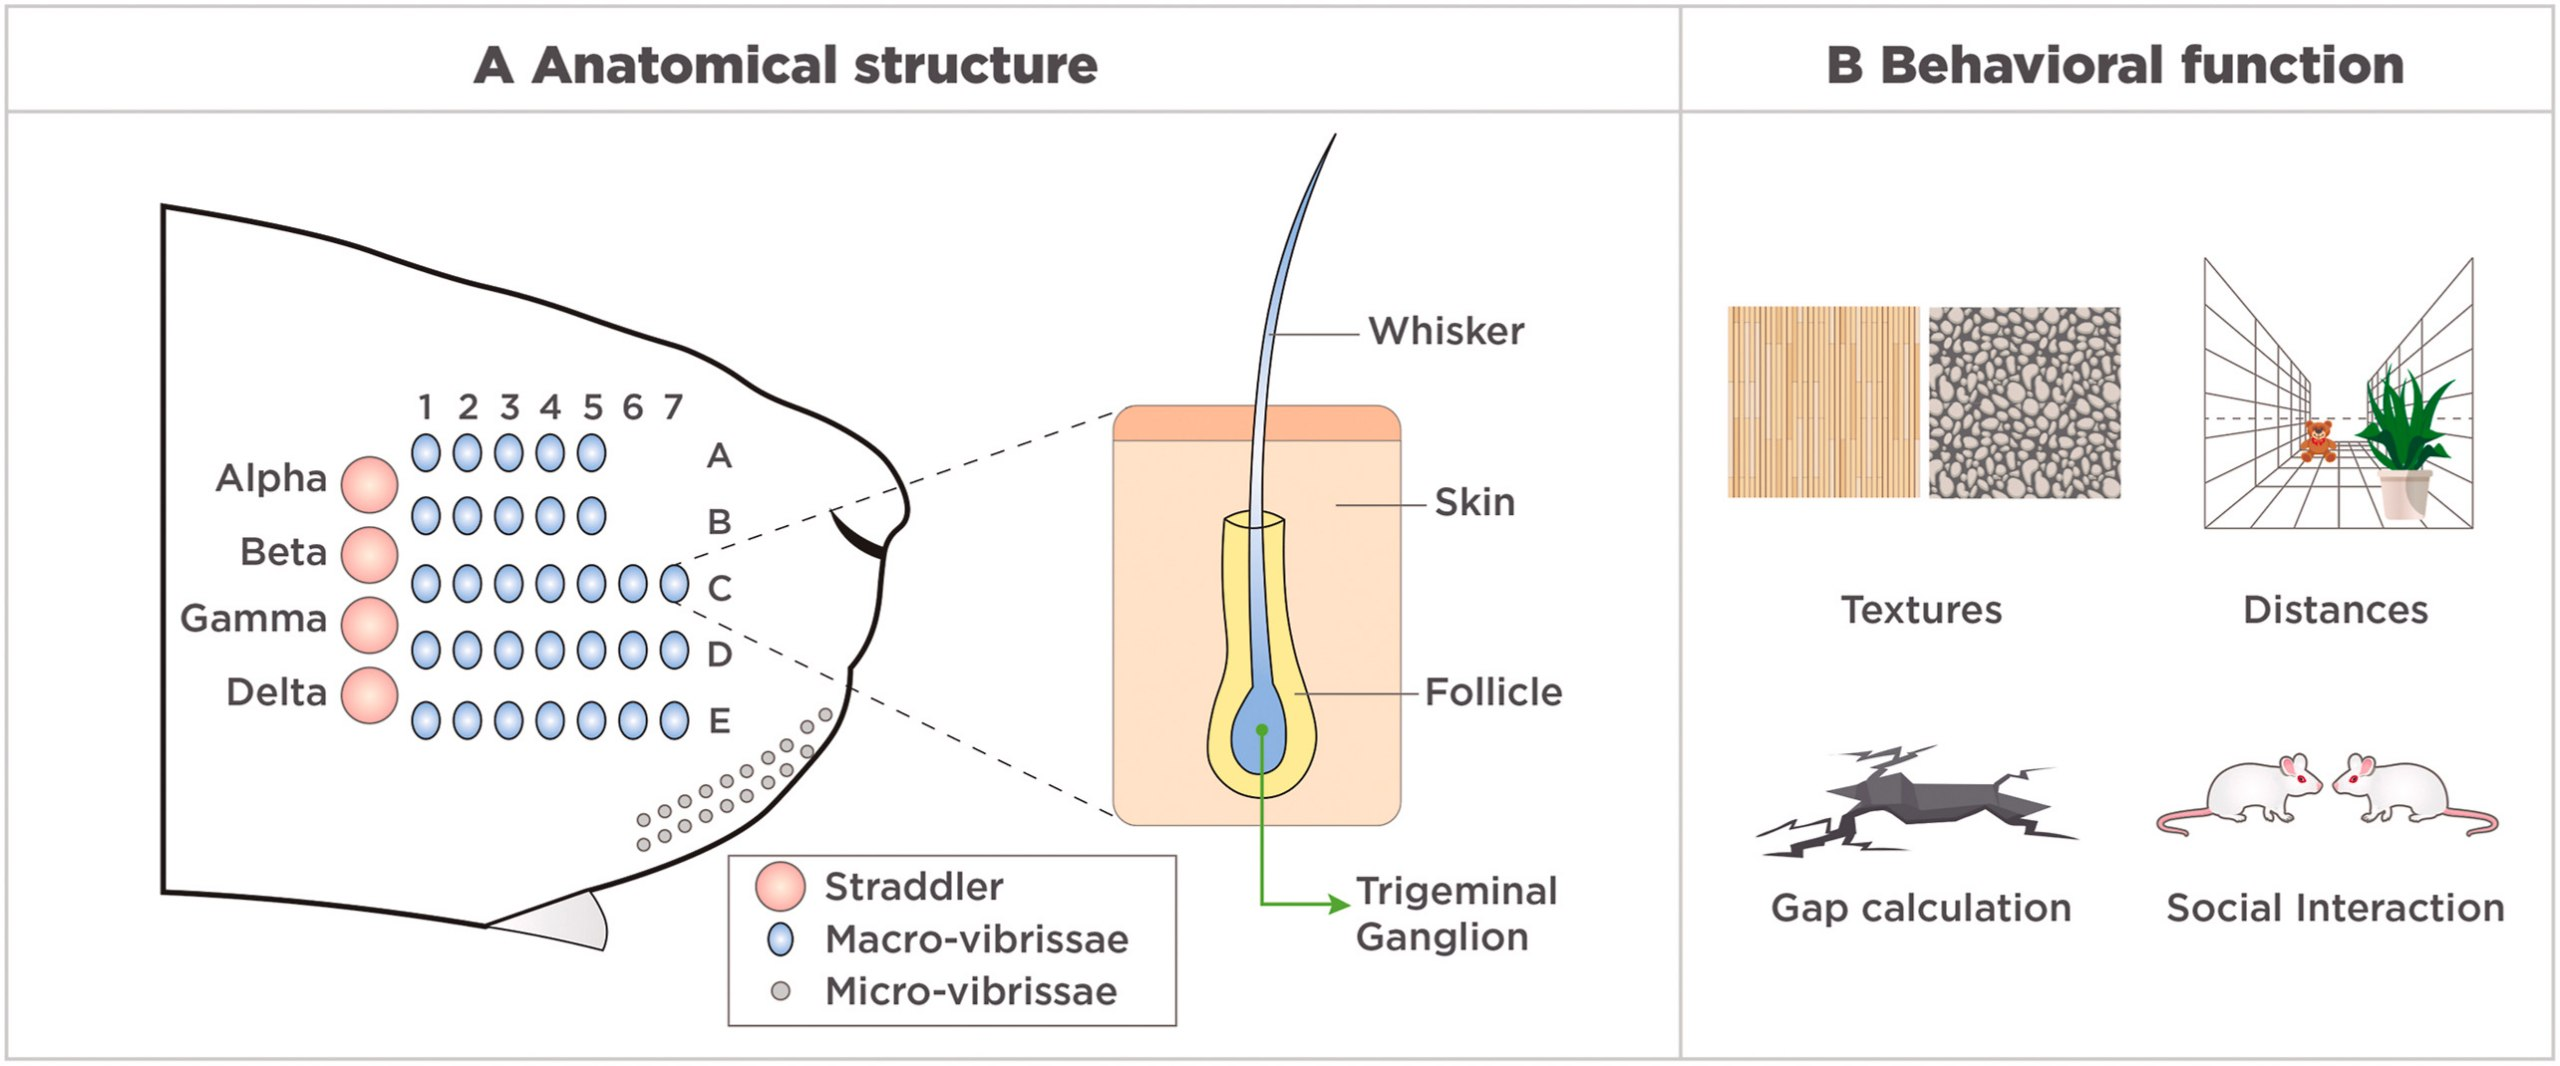
\includegraphics[width=\textwidth]{figures/whisker-anatomy}
    \caption{Representation of the vibrissae system and its function, from~\cite{IBARRACASTANEDA2022100034}}
\end{figure}


\section{Robotic Whisker Sensors}

\begin{itemize}
    \item Strain gauge: bending \to strain detection.
    \item Magnetic (Hall): bending \to magnetic shift.
    \item Optical: deflection \to light variation.
\end{itemize}
\begin{figure}[htb]
    \centering
    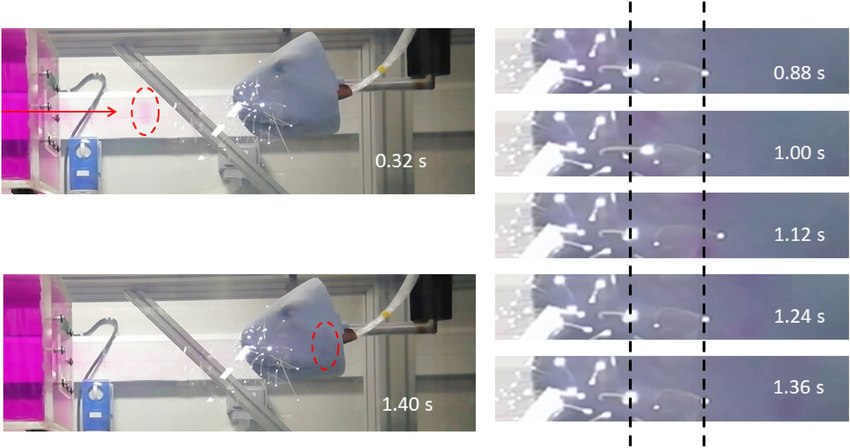
\includegraphics[height=0.5\textheight]{figures/optical-whisker}
    \caption{Picture of the 3D printed sea lion head with integrated optical whiskers, from \cite{optical-whisker}}
\end{figure}


\section{Whisker Sensor Applications}

Prominent applications according to~\cite{s22072705}:
\begin{itemize}
    \item Biomimetic tactile: prosthetic feedback via impedance sensing.
    \item Robotic spatial sensing: 3D object localization and environmental mapping.
    \item Surface texture analysis: mapping surface details through whisking data.
    \item Navigation in dark: autonomous whisking for low-light environments.
    \item Underwater sensing: flow detection and vortex vibration control.
\end{itemize}

